%% LyX 2.2.3 created this file.  For more info, see http://www.lyx.org/.
%% Do not edit unless you really know what you are doing.
\documentclass[english,12pt]{article}
\usepackage[T1]{fontenc}
\usepackage[latin9]{inputenc}
\usepackage{mathtools}
\usepackage{amsmath}
\usepackage{amsthm}
\usepackage{amssymb}
\usepackage{graphicx}

\makeatletter
%%%%%%%%%%%%%%%%%%%%%%%%%%%%%% Textclass specific LaTeX commands.
\theoremstyle{plain}
\newtheorem{thm}{\protect\theoremname}[section]
\theoremstyle{definition}
\newtheorem{defn}[thm]{\protect\definitionname}
\theoremstyle{plain}
\newtheorem{prop}[thm]{\protect\propositionname}
\ifx\proof\undefined
\newenvironment{proof}[1][\protect\proofname]{\par
\normalfont\topsep6\p@\@plus6\p@\relax
\trivlist
\itemindent\parindent
\item[\hskip\labelsep\scshape #1]\ignorespaces
}{%
\endtrivlist\@endpefalse
}
\providecommand{\proofname}{Proof}
\fi
\theoremstyle{definition}
\newtheorem{example}[thm]{\protect\examplename}

%%%%%%%%%%%%%%%%%%%%%%%%%%%%%% User specified LaTeX commands.
\usepackage[margin=1in]{geometry}
\usepackage{tikz}
\usetikzlibrary{arrows,decorations.pathreplacing,shapes}

\makeatother

\usepackage{babel}
\providecommand{\definitionname}{Definition}
\providecommand{\examplename}{Example}
\providecommand{\propositionname}{Proposition}
\providecommand{\theoremname}{Theorem}

\begin{document}

\title{Math 525: Lecture 21}

\date{March 29, 2018}

\maketitle
So far, we have worked primarily with (stationary) Markov chains whose
transition matrices are ``constant''. In this lecture, we explore
the following question: what if we could ``control'' the transition
matrix? In this context, we will have a transition matrix $P(\pi)$
that depends on some quantity $\pi$ which we, the ``controller'',
get to choose.

\section{Markov decision processes}

For this lecture, our setting is as follows:
\begin{itemize}
\item $S=\{1,\ldots,m\}$ is a finite state space.
\item To each state $i$ in $S$ is associated a nonempty countable set
$\mathcal{A}_{i}$ which we can intuitively think of as all the ``actions''
available at state $i$.
\end{itemize}
\begin{defn}
A \emph{stationary policy} $\pi_{0}$ is a function whose domain is
$S$ and which satisfies $\pi_{0}(i)\in\mathcal{A}_{i}$ for all $i$.
The set of all stationary policies is denoted $\Pi_{0}$
\end{defn}
%
\begin{defn}
A \emph{randomized policy} $(\pi_{n})_{n\geq0}$ is a sequence in
which each $\pi_{n}(i)$ is a random variable satisfying
\begin{itemize}
\item $\pi_{n}(i)$ takes values in $\mathcal{A}_{i}$ a.s. and
\item $\{\pi_{n}(i)=a\}\in\mathcal{F}_{n}$ for each $a$ in $\mathcal{A}_{i}$.
\end{itemize}
The set of all randomized policies is denoted $\Pi$. 
\end{defn}
For each state $i$ in $S$ and action $a$ in $\mathcal{A}_{i}$,
let $p_{i}(a)$ denote a nonnegative column vector satisfying $p_{i}(a)^{\intercal}e=1$.
Given a randomized policy $\pi$, let $(X_{n}^{\pi})_{n\geq0}$ denote
a Markov chain satisfying
\[
\mathbb{P}(X_{n+1}^{\pi}=j\mid X_{n}^{\pi}=i)=p_{i}(\pi_{n}(i))^{\intercal}e_{j}.
\]
That is, the transition matrix at time $n$ is 
\[
P(\pi_{n})=\begin{pmatrix}p_{1}(\pi_{n}(1))^{\intercal}\\
p_{2}(\pi_{n}(2))^{\intercal}\\
\vdots\\
p_{m}(\pi_{n}(m))^{\intercal}
\end{pmatrix}.
\]

Now, let $c:S\rightarrow\mathbb{R}$, $0\leq d<1$, and
\begin{equation}
J(i,\pi)=\mathbb{E}\left[\sum_{n\geq0}d^{n}c(X_{n}^{\pi})\middle|X_{0}^{\pi}=i\right].\label{eq:objective}
\end{equation}
We can think of
\begin{itemize}
\item $c(X_{n}^{\pi})$ as the cost incurred at time $n$ and
\item $d^{n}$ as a discount factor which attempts to capture the fact that
costs incurred in the ``future'' are not as bad as costs incurred
``today''.
\end{itemize}
Our objective is to pick $\pi$ so as to minimize $J(i,\pi)$. That
is, we are interested in the quantity
\begin{equation}
\boxed{v(i)=\inf_{\pi\in\Pi}J(i,\pi)}\label{eq:mdp}
\end{equation}
We call (\ref{eq:mdp}) a \emph{Markov decision process} (MDP).
\begin{prop}
$v(i)$ is bounded for each $i$.
\end{prop}
\begin{proof}
This is a trivial consequence of the discount factor being strictly
less than one:
\[
\left|v(i)\right|\leq\sum_{n\geq0}d^{n}\max_{j}\left|c(j)\right|=\frac{1}{1-d}\max_{j}\left|c(j)\right|.\qedhere
\]
\end{proof}

\section{Dynamic programming}

By the Markov property,
\begin{multline*}
J(i,\pi)=\mathbb{E}^{i}\left[c(X_{0}^{\pi})+\sum_{n\geq1}d^{n}c(X_{n}^{\pi})\right]=c(i)+d\mathbb{E}^{i}\left[\sum_{n\geq0}d^{n}c(X_{n+1}^{\pi})\right]\\
=c(i)+d\mathbb{E}^{i}\left[J(X_{1}^{\pi},(\pi_{n})_{n\geq1})\right]\geq c(i)+d\sum_{j}(P(\pi_{0}))_{ij}v(j)
\end{multline*}
where $\pi_{0}$ is some stationary policy. Taking infimums of both
sides of this equality,
\begin{equation}
v(i)\geq\inf_{\pi_{0}\in\Pi_{0}}\left\{ c(i)+d\sum_{j}(P(\pi_{0}))_{ij}v(j)\right\} .\label{eq:ldp}
\end{equation}

Now, fix $\epsilon>0$. For each $i$, let $\pi^{i}=(\pi_{n}^{i})_{n\geq0}$
be a randomized policy which satisifes
\[
v(i)\geq J(i,\pi^{i})+\epsilon.
\]
Let $\pi_{0}$ be an arbitrary stationary policy. Define a new randomized
policy $\pi^{\epsilon}=(\pi_{n}^{\epsilon})_{n\geq0}$ by
\[
\pi_{n}^{\epsilon}=\begin{cases}
\pi_{0} & \text{if }n=0\\
\sum_{i}\mathbf{1}_{\{X_{1}^{\pi_{0}}=i\}}\pi_{n-1}^{i} & \text{if }n>0.
\end{cases}
\]
Note that
\[
v(i)\leq J(i,\pi^{\epsilon})=c(i)+d\sum_{j}(P(\pi_{0}))_{ij}J(j,\pi^{j})\leq c(i)+d\sum_{j}(P(\pi_{0}))_{ij}v(j)-\epsilon.
\]
Now, take infimums of both sides to get
\begin{equation}
v(i)\leq\inf_{\pi_{0}\in\Pi_{0}}\left\{ c(i)+d\sum_{j}(P(\pi_{0}))_{ij}v(j)\right\} -\epsilon.\label{eq:udp}
\end{equation}

We can take $\epsilon\downarrow0$ and combine (\ref{eq:ldp}) and
(\ref{eq:udp}) to arrive at 
\begin{equation}
v(i)=\inf_{\pi_{0}\in\Pi_{0}}\left\{ c(i)+d\sum_{j}(P(\pi_{0}))_{ij}v(j)\right\} .\label{eq:dp}
\end{equation}
The implications of this are amazing! We started out with an objective
function (\ref{eq:objective}) that was daunting: minimizing it would
require picking a stationary policy for each time $n$. However, we
were able to use the Markov property to reduce this to a ``local''
problem that only involves minimizing over all stationary policies
$\pi_{0}$. In fact, we can simplify (\ref{eq:dp}) even further.
First, we need some notation:
\[
\text{for }\{y_{\alpha}\}_{\alpha}\in\mathbb{R}^{n}\text{, }\inf_{\alpha}y_{\alpha}\text{ is the vector with entries }\inf_{\alpha}(y_{\alpha})_{i}.
\]
\begin{thm}[Dynamic programming]
Let $v=(v(1),\ldots,v(m))^{\intercal}$ and $c=(c(1),\ldots,c(m))^{\intercal}$
where $v(i)$ is the quantity defined by (\ref{eq:mdp}). Then,
\[
\boxed{\sup_{\pi_{0}\in\Pi_{0}}\left\{ \left(I-dP(\pi_{0})\right)v-c\right\} =0}
\]
\end{thm}
\begin{proof}
We can rewrite (\ref{eq:dp}) as
\begin{equation}
v=\inf_{\pi_{0}\in\Pi}\left\{ c+dP(\pi_{0})v\right\} .\label{eq:fixpoint}
\end{equation}
Moving some terms around, we obtain the desired result.
\end{proof}
In fact, the situation is much more general than we have let on. We
can allow for more general discount factors and costs:
\[
J(i,\pi)=\mathbb{E}\left[\sum_{n\geq0}d(\pi_{n},X_{n}^{\pi})^{n}c(\pi_{n},X_{n}^{\pi})\middle|X_{0}^{\pi}=i\right].
\]
However, in this case, it is no longer necessarily the case that $v(\cdot)$
is bounded. When it is, the corresponding dynamic programming equation
is
\begin{equation}
\sup_{\pi_{0}\in\Pi_{0}}\left\{ \left(I-D(\pi_{0})P(\pi_{0})\right)v-c(\pi_{0})\right\} =0\label{eq:dp_general}
\end{equation}
where $D(\pi_{0})=\operatorname{diag}(d(\pi_{0}(1),1),\ldots,d(\pi_{0}(m),m))$
and $c(\pi_{0})=(c(\pi_{0}(1),1),\ldots,c(\pi_{0}(m),m))^{\intercal}$.

In light of this, the remainder of this lecture is focused on (\ref{eq:dp_general}).
In particular, we would like to know if an arbitrary vector $v$ satisfies
(\ref{eq:dp_general}), is it necessarily equal to the MDP (\ref{eq:mdp})?
Moreover, can we use (\ref{eq:dp_general}) to compute the MDP?

\section{Matrix classes}

First, we will need to recall some more linear algebra.

\subsection{Monotone matrices}
\begin{defn}
A \emph{monotone matrix} is a real square matrix $A$ such that $Ax\geq0$
implies $x\geq0$ for all real vectors $x$.
\end{defn}
\begin{prop}
Monotone matrices are nonsingular.
\end{prop}
\begin{proof}
Let $A$ be a monotone matrix and assume there exists $x$ with $Ax=0$.
Then, by monotonicity, $x\geq0$ and $-x\geq0$, and hence $x=0$.
\end{proof}
%
\begin{prop}
A real square matrix $A$ is monotone if and only if $A^{-1}$ exists
and is nonnegative.
\end{prop}
\begin{proof}
Suppose $A$ is monotone. Denote by $x$ the $i$-th column of $A$.
Then, $Ax$ is the $i$-th standard basis vector, and hence $x\geq0$
by monotonicity. For the reverse direction, suppose $A$ admits a
nonnegative inverse. Then, if $Ax\geq0$, $x=A^{-1}Ax\geq A^{-1}0=0$,
and hence $A$ is monotone.
\end{proof}

\subsection{M-matrices}
\begin{defn}
An \emph{M-matrix} is any square matrix $A$ which can be written
in the form
\begin{equation}
A=sI-B\label{eq:m_matrix}
\end{equation}
where $s\geq\rho(B)$ and $B$ is nonnegative.
\end{defn}
\begin{prop}
The M-matrix (\ref{eq:m_matrix}) is nonsingular if and only if $s>\rho(B)$.
\end{prop}
\begin{proof}
Note that $A$ is nonsingular if and only if $s$ is an eigenvalue
of $B$ since
\[
Ax=sx-Bx=0\iff Bx=sx.
\]
Therefore, if $s>\rho(B)$, then $A$ is nonsingular. Conversely,
if $s=\rho(B)$, by the Perron-Frobenius theorem, $s$ is an eigenvalue
of $B$.
\end{proof}
\begin{prop}
Nonsingular M-matrices are monotone.
\end{prop}
\begin{proof}
Divide (\ref{eq:m_matrix}) by $s$ so that
\[
s^{-1}A=I-s^{-1}B.
\]
Noting that $\rho(s^{-1}B)<1$, the inverse of the right hand side
of the above is the Neumann series
\[
\left(I-s^{-1}B\right)^{-1}=\sum_{k\geq0}\left(s^{-1}B\right)^{k}.
\]
In particular, this Neumann series consists only of powers of nonnegative
matrices, and therefore converges to a nonnegative matrix. In other
words, $sA^{-1}$ is nonnegative, and hence so too is $A^{-1}$. 
\end{proof}

\subsection{Weakly chained diagonally dominant matrices}
\begin{defn}
Let $A=(A_{ij})$ be a matrix. We say its $i$-th row is \emph{strictly
diagonally dominant} (s.d.d.) if
\begin{equation}
\left|A_{ii}\right|>\sum_{i\neq j}\left|A_{ij}\right|.\label{eq:sdd}
\end{equation}
We say the matrix is s.d.d. if all of its rows are s.d.d. Weakly diagonally
dominant (w.d.d.) is defined with weak inequality ($\geq$) instead.
\end{defn}
\begin{example}
The matrix
\begin{equation}
\begin{pmatrix}\phantom{-}1\\
-1 & \phantom{-}1\\
 & -1 & \phantom{-}1\\
 &  & -1 & \phantom{-}1
\end{pmatrix}\label{eq:matrix}
\end{equation}
is not strictly diagonally dominant, but it is weakly diagonally dominant.
\end{example}
\begin{defn}
\label{def:wcdd}Let $A=(A_{ij})$ be a matrix. Let \[ J = \{ i \colon i \text{ satisfies } \eqref{eq:sdd} \} \]
denote the set of all s.d.d. rows of $A$. We say $A$ is \emph{weakly
chained diagonally dominant} (w.c.d.d.) if
\begin{enumerate}
\item $A$ is w.d.d.
\item \label{enu:wcdd}For each row $i\notin J$, there is a walk $i\rightarrow j$
with $j\in J$.
\end{enumerate}
\end{defn}
\begin{example}
The matrix (\ref{eq:matrix}) is w.c.d.d. (see Figure \ref{fig:graph}).
\end{example}
\begin{figure}
\begin{centering}
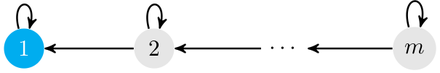
\includegraphics[width=3in]{wcdd}
\par\end{centering}
\caption{Graph of (\ref{eq:matrix})\label{fig:graph}}
\end{figure}
\begin{prop}
w.c.d.d. matrices are nonsingular.\footnote{Shivakumar, P. N., and Kim Ho Chew. \textquotedbl{}A sufficient condition
for nonvanishing of determinants.\textquotedbl{} Proceedings of the
American mathematical society (1974): 63-66.}
\end{prop}
\begin{proof}
Let $A$ be w.c.d.d. If $A$ is singular, we can find a nonzero vector
$x$ such that $Ax=0$. Without loss of generality, let $i_{1}$ be
such that $|x_{i_{1}}|=1\geq|x_{j}|$ for all $j$. Since $A$ is
w.c.d.d., we may pick a walk $i_{1}\dashrightarrow i_{2}\dashrightarrow\cdots\dashrightarrow i_{k}$
ending at an s.d.d. row $i_{k}\in J$.

Taking moduli on both sides of
\[
-a_{i_{1}i_{1}}x_{i_{1}}=\sum_{j\neq i_{1}}a_{i_{1}j}x_{j}
\]
yields
\[
\left|a_{i_{1}i_{1}}\right|=\left|a_{i_{1}i_{1}}x_{i_{1}}\right|=\left|\sum_{j\neq i_{1}}a_{i_{1}j}x_{j}\right|\leq\sum_{j\neq i_{1}}\left|a_{i_{1}j}\right|\left|x_{j}\right|\leq\sum_{j\neq i_{1}}\left|a_{i_{1}j}\right|.
\]
Since $A$ is w.d.d., the above must hold with equality. Therefore,
$|x_{j}|=1$ whenever $a_{i_{1}j}$ is nonzero. In particular, $|x_{i_{2}}|=1$,
and we can repeat the same argument as above to get that row $i_{2}$
is not s.d.d., row $i_{3}$ is not s.d.d., etc. until we conclude
that row $i_{k}$ is not s.d.d., a contradiction.
\end{proof}

\subsubsection*{To be continued...}
\end{document}
